\documentclass[11pt]{article}

\newcommand{\yourname}{Gabriel Peter}
\newcommand{\yourcollaborators}{}

\def\comments{0}

%format and packages

%\usepackage{algorithm, algorithmic}
\usepackage{algpseudocode}
\usepackage{amsmath, amssymb, amsthm}
\usepackage{enumerate}
\usepackage{enumitem}
\usepackage{framed}
\usepackage{verbatim}
\usepackage{listings}
\usepackage[margin=1.0in]{geometry}
\usepackage{microtype}
\usepackage{multirow}
\usepackage{kpfonts}
\usepackage{palatino}
	\DeclareMathAlphabet{\mathtt}{OT1}{cmtt}{m}{n}
	\SetMathAlphabet{\mathtt}{bold}{OT1}{cmtt}{bx}{n}
	\DeclareMathAlphabet{\mathsf}{OT1}{cmss}{m}{n}
	\SetMathAlphabet{\mathsf}{bold}{OT1}{cmss}{bx}{n}
	\renewcommand*\ttdefault{cmtt}
	\renewcommand*\sfdefault{cmss}
	\renewcommand{\baselinestretch}{1.06}
\usepackage[usenames,dvipsnames]{xcolor}
\definecolor{DarkGreen}{rgb}{0.15,0.5,0.15}
\definecolor{DarkRed}{rgb}{0.6,0.2,0.2}
\definecolor{DarkBlue}{rgb}{0.2,0.2,0.6}
\definecolor{DarkPurple}{rgb}{0.4,0.2,0.4}
\usepackage[pdftex]{hyperref}
\hypersetup{
	linktocpage=true,
	colorlinks=true,				% false: boxed links; true: colored links
	linkcolor=DarkBlue,		% color of internal links
	citecolor=DarkBlue,	% color of links to bibliography
	urlcolor=DarkBlue,		% color of external links
}

\usepackage[boxruled,vlined,nofillcomment]{algorithm2e}
	\SetKwProg{Fn}{Function}{\string:}{}
	\SetKwFor{While}{While}{}{}
	\SetKwFor{For}{For}{}{}
	\SetKwIF{If}{ElseIf}{Else}{If}{:}{ElseIf}{Else}{:}
	\SetKw{Return}{Return}

\usepackage{tikz}
	\usetikzlibrary{positioning}
	\definecolor{processblue}{cmyk}{0.96,0,0,0}
    \usetikzlibrary{matrix,arrows}

	

%enclosure macros
\newcommand{\paren}[1]{\ensuremath{\left( {#1} \right)}}
\newcommand{\bracket}[1]{\ensuremath{\left\{ {#1} \right\}}}
\renewcommand{\sb}[1]{\ensuremath{\left[ {#1} \right\]}}
\newcommand{\ab}[1]{\ensuremath{\left\langle {#1} \right\rangle}}

%probability macros
\newcommand{\ex}[2]{{\ifx&#1& \mathbb{E} \else \underset{#1}{\mathbb{E}} \fi \left[#2\right]}}
\newcommand{\pr}[2]{{\ifx&#1& \mathbb{P} \else \underset{#1}{\mathbb{P}} \fi \left[#2\right]}}
\newcommand{\var}[2]{{\ifx&#1& \mathrm{Var} \else \underset{#1}{\mathrm{Var}} \fi \left[#2\right]}}


%useful CS macros
\newcommand{\poly}{\mathrm{poly}}
\newcommand{\polylog}{\mathrm{polylog}}
\newcommand{\zo}{\{0,1\}}
\newcommand{\pmo}{\{\pm1\}}

\newcommand{\getsr}{\gets_{\mbox{\tiny R}}}
\newcommand{\card}[1]{\left| #1 \right|}
\newcommand{\set}[1]{\left\{#1\right\}}
\newcommand{\negl}{\mathrm{negl}}
\newcommand{\eps}{\varepsilon}
\DeclareMathOperator*{\argmin}{arg\,min}
\DeclareMathOperator*{\argmax}{arg\,max}
\newcommand{\eqand}{\qquad \textrm{and} \qquad}
\newcommand{\ind}[1]{\mathbb{I}\{#1\}}
\newcommand{\sslash}{\ensuremath{\mathbin{/\mkern-3mu/}}}

%mathbb
\newcommand{\N}{\mathbb{N}}
\newcommand{\R}{\mathbb{R}}
\newcommand{\Z}{\mathbb{Z}}
%mathcal
\newcommand{\cA}{\mathcal{A}}
\newcommand{\cB}{\mathcal{B}}
\newcommand{\cC}{\mathcal{C}}
\newcommand{\cD}{\mathcal{D}}
\newcommand{\cE}{\mathcal{E}}
\newcommand{\cF}{\mathcal{F}}
\newcommand{\cL}{\mathcal{L}}
\newcommand{\cM}{\mathcal{M}}
\newcommand{\cO}{\mathcal{O}}
\newcommand{\cP}{\mathcal{P}}
\newcommand{\cQ}{\mathcal{Q}}
\newcommand{\cR}{\mathcal{R}}
\newcommand{\cS}{\mathcal{S}}
\newcommand{\cU}{\mathcal{U}}
\newcommand{\cV}{\mathcal{V}}
\newcommand{\cW}{\mathcal{W}}
\newcommand{\cX}{\mathcal{X}}
\newcommand{\cY}{\mathcal{Y}}
\newcommand{\cZ}{\mathcal{Z}}

%theorem macros
\newtheorem{thm}{Theorem}
\newtheorem{lem}[thm]{Lemma}
\newtheorem{fact}[thm]{Fact}
\newtheorem{clm}[thm]{Claim}
\newtheorem{rem}[thm]{Remark}
\newtheorem{coro}[thm]{Corollary}
\newtheorem{prop}[thm]{Proposition}
\newtheorem{conj}[thm]{Conjecture}

\theoremstyle{definition}
\newtheorem{defn}[thm]{Definition}

\usepackage{mathtools}
\DeclarePairedDelimiter{\ceil}{\lceil}{\rceil}


\newcommand{\instructor}{Drew van der Poel}
\newcommand{\hwnum}{5}
\newcommand{\hwdue}{Friday, June 18 at 11:59pm via \href{https://gradescope.com/courses/266585}{Gradescope}}

\theoremstyle{theorem}
\newtheorem{prob}{Problem}
\newtheorem{sol}{Solution}

\definecolor{cit}{rgb}{0.05,0.2,0.45} 
\newcommand{\solution}{\medskip\noindent{\color{DarkBlue}\textbf{Solution:}}}

\begin{document}
{\Large 
\begin{center}{CS3000: Algorithms \& Data} --- Summer I '21 --- \instructor \end{center}}
{\large
\vspace{10pt}
\noindent Homework~\hwnum \vspace{2pt}\\
Due~\hwdue}

\bigskip
{\large
\noindent Name: \yourname \vspace{2pt}\\ Collaborators: \yourcollaborators}

\vspace{15pt}
\begin{itemize}

\item Make sure to put your name on the first page.  If you are using the \LaTeX~template we provided, then you can make sure it appears by filling in the \texttt{yourname} command.

\item This assignment is due~\hwdue.  No late assignments will be accepted.  Make sure to submit something before the deadline.

\item Solutions must be typeset in \LaTeX.  If you need to draw any diagrams, you may draw them by hand as long as they are embedded in the PDF.  I recommend using the source file for this assignment to get started.

\item I encourage you to work with your classmates on the homework problems. \emph{If you do collaborate, you must write all solutions by yourself, in your own words.}  Do not submit anything you cannot explain.  Please list all your collaborators in your solution for each problem by filling in the \texttt{yourcollaborators} command.

\item Finding solutions to homework problems on the web, or by asking students not enrolled in the class is strictly forbidden.

\end{itemize}

\newpage

\begin{prob} No one man should have all that power \emph{(26 points)}\end{prob}

You work for a public relations firm and have acquired complete
information on the post-election Washington DC lobbying network.  In
particular, you have a list $V$ of $n$ persons (congressmen,
bureaucrats, lobbyists, businessmen, etc.) and for each person $i$ in
$V$, a list of persons in $V$ that $i$ can {\em influence}.  (Note
that it is possible that $i$ can influence $j$ but $j$ cannot
influence $i$.)

Having just studied graph algorithms, you immediately capture the
above information by a directed graph $G$ with $V$ as the set of
vertices and the set $E$ of edges defined as follows.
\[
E = \{(i,j): i \mbox{ can influence } j\}.
\]

Call a person $i$ a {\em powerbroker}\/ if for every other person $j
\in V$, there is a path from $i$ to $j$ in $G$.


\begin{enumerate}[label=(\alph*)]
\item[{\bf (a)}]  \textbf{(4 points)} Give an example lobbying network with five persons in
  which there are exactly three powerbrokers.

\solution \\ 
\begin{figure}[h!]
	\begin{center}
	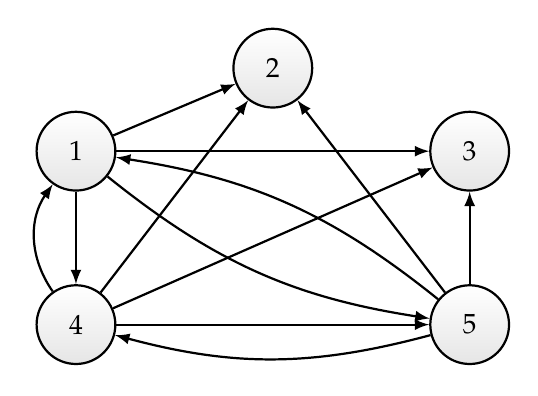
\begin{tikzpicture}[>= latex, node distance = 1.5 cm and 2.5cm,on grid, thick,state/.style ={circle,top color =white,bottom color = gray!20,draw,black,text=black,minimum width =1.0 cm}]
	\node[state] (a) {1};
	\node[state] (b) [yshift=30pt, right =of a] {2};
	\node[state] (c) [yshift=-30pt, right =of b] {3};
	% \node[state] (d) [below =of a, yshift=-10] {d};
	% \node[state] (e) [right =of d] {e};
	% \node[state] (f) [right =of e] {f};
	\node[state] (g) [below =of a, yshift=-20] {4};
	% \node[state] (h) [right =of g] {h};
	\node[state] (i) [right =of g, below= of c, yshift=-20] {5};
	\tikzset{every node/.style={fill=white}} 
	\path[->] 	
			(a) edge  				(b)
			(a) edge				(c)
			(a) edge				(g)
			(a) edge [bend right=15]	(i)
			(g) edge	[bend left=35]			(a)

			(g) edge				(b)
			(g) edge				(c)
			(g) edge				(i)
			(i) edge		[bend left=15]		    (g)

			(i) edge				(c)
			(i) edge				(b)
			(i) edge	[bend right=15]			(a)
			;
	\end{tikzpicture}
	\end{center}
	\end{figure}


\item[{\bf (b)}] Design and analyze a polynomial-time algorithm to
  determine {\em all}\/ powerbrokers in the given lobbying network.
  If there are no powerbrokers, then your algorithm must indicate so.

  \begin{enumerate}[label=(\roman*)]
  \item  \textbf{(2 points)} Describe precisely what your algorithm is given as input and
    what it needs to output.\footnote{\textbf{Check:} Make sure you
      have this right, before you move on to designing the algorithm.}

\solution \\

The algorithm simply needs a provided graph in the form of adjacency lists. It will then output a list of the vertices that compose the list of powerbrokers (aka the source SCC, which will be explained later.)

    
  \item  \textbf{(8 points)} Describe your algorithm.  You may invoke or
    modify any of the graph traversal algorithms studied in class.

\solution \\

\lstinputlisting[language=Python]{1_pseudo.py}
This algorithm goes under the basis that all powerbrokers will be in a SCC. Additionally, if these vertices need to have possible paths to all other nodes, then we can also be confident that this is a sink component. (more in iii.) \\\\
Thus, we first need to find all SCCs using inspiration for the linear-time algorithm discussed in class. Based on the nature of the alogrithm, which disvoers the sink components first, we know that the last SCC is the source and therefore contains the power brokers.

  \item \textbf{(8 points)}
    Justify the correctness of your algorithm.  Your justification does
    not need to be long or formal, just convincing.

\solution \\ 

As mentioned before, we can be certain that all powerbrokers are in the same SCC because they must be connected to each in order to satisfy the requirement that:\\\\
"Call a person $i$ a {\em powerbroker}\/ if for every other person $j
\in V$, there is a path from $i$ to $j$ in $G$."\\\\
Additionally, the SCC in question must be the source SCC because a source component, has a path to all other nodes which is necesarry for a power broker.\\\\
Therfore, {powerbrokers} $\leftrightarrow SCC_{source}$ 

  \item  \textbf{(4 points)} Analyze the running time of your algorithm in terms of the
    number of vertices $n$ and number of edges $m$ of $G$.

    (Any correct polynomial-time algorithm will suffice to get full
    credit.  See if you can design an algorithm with $O(n + m)$
    running time using strongly connected components.)

\solution \\

The runtime of this algorithm is identical to the SCC mentioned in class, but simply more things are cached for later reference:\\\\
\begin{enumerate}
	\item tranposing the graph: $O(m)$
	\item DFS on the tranposed: $O(n + m)$
	\item comp init: $O(n)$
	\item Nested for-loops assigning SCC's to vertices: $O(n + m)$
\end{enumerate}

TOTAL: $O(m) + O(n + m) + O(n) + O(n + m) = O(n + m)$

  \end{enumerate}
\end{enumerate}

\newpage



\begin{prob}Stagecraft  \emph{(24+5 points)}\end{prob}

You're in charge of assembling the stage for this year's \emph{AlgoRhythms Music Festival (starring Master P).}  Assembling the stage in time will require careful planning.  You are given:
\begin{itemize}
\item A set $V$ of $n$ small tasks that are required to complete the stage.
\item A set $E$ of pairs of tasks in $V$. A pair $(u,v)$ is in $E$ if task $u$ must be completed before task $v$ is started. There are no cycles in $E.$
\item For each task $u \in V$, the amount of time $t(u)$ required for the task.
\end{itemize}
You have a very large team, so you can work on any number of tasks in parallel, but you cannot start a task $u$ until all of the prerequisite tasks $v$ have been completed.

Design an algorithm that takes as input the graph $G = (V,E)$ (represented as an adjacency list) and the time for each task, and outputs a list consisting of the earliest possible time that each task can be completed.  An example of a correct input-output is:


\begin{table}[h!]
\centering
\begin{tabular}{lll}
\multicolumn{2}{c}{\textbf{Input:}\vspace{3pt}}       & \multicolumn{1}{c}{~~~~~~~~~~~~~~\textbf{Output:}} \\
$t(1) = 10$ & \multirow{4}{*}{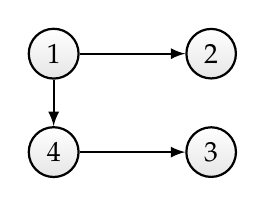
\begin{tikzpicture}[>= latex,node distance = 1.25 cm and 2.0cm,on grid, thick,state/.style ={circle,top color =white,bottom color = gray!20,draw,black,text=black,minimum width =.2 cm}]
\node[state] (a) {1};
\node[state] (b) [right =of a] {2};
\node[state] (c) [below =of b] {3};
\node[state] (d) [below =of a] {4};
\path[->] 	(a) edge node {} (b)
				(a) edge node {} (d);
\path[->]	(d) edge node {} (c);
\end{tikzpicture}} & ~~~~~~~~~~~~~~$c(1) = 10$                \\
$t(2) = 11$ &                   & ~~~~~~~~~~~~~~$c(2) = 21$                \\
$t(3) = 8$  &                   & ~~~~~~~~~~~~~~$c(3) = 23$                \\
$t(4) = 5$  &                   & ~~~~~~~~~~~~~~$c(4) = 15$               
\end{tabular}
\end{table}

Your algorithm should run in $O(n+m)$ time.

\begin{enumerate}[label=(\alph*)]
\item  \textbf{(6 points)} Describe in 1-3 English sentences how you will determine the earliest possible completion times for the tasks.

\solution \\ I will determine the the earliest possible completion of each node by running a modified DFS algorithm
for topological sorting, which has an additional modification that labels each node's topology as their cumulative time weights such that we keep track of the current max accumulation of times for a DFS.

\item  \textbf{(6 points)} Describe your algorithm in pseudocode.  You may make use of any algorithm we've seen in class without describing how it works, but you should clearly state what you are assuming about the algorithm.

\solution \\

\lstinputlisting[language=Python]{2.py}
The algorithm works very similar to the FastTop() mentioned in lecture 16:\\

Essentially, we remove all nodes and then add their accumulated time to complete starting at the nodes
with 0 in-degree edges. By deleting nodes, we cause others to now have 0 in-degrees and are then deleted as well. The topological times are 
a max of the current label or the new accumulation, which denotes the soonest this node (task) can be completed after all prerequisites are finished.
The labelings are stored in a map: `times` and from there can be easily acessed such that: $c(i) = times[i]$


\item   \textbf{(8 points)} Justify that your algorithm outputs the earliest possible completion time for each project.  Your justification can take any form you like as long as the argument is clear and logical.

\solution \\ 

Theorem: G has a topological ordering $\leftrightarrow$ G is a DAG\\

As that is a provided contraint of the graph input, that it is a acyclic DAG. We know that we can get a topological ordering. 
In a normal topological sort, know that we can get a list which is a guaranteed precedence ordering of the nodes provided.
I alter that algorithm ever-so-slighty to maintain its correctness of topological order, but labeling them through an accumulation of their $t(i)$ value.
We know based on the alogrithm that the accumulation will only be passed to nodes that are in the precendence of the currently deleting node,
as the next-to-be deleted are out\_degrees of it. However, based on the configuration of the graph, we may have multiple precedences for a single node,
and this causes a value conflict in out labeling. To solve this, we take the max(old accumulation, new accumulation) as the problem constraints mentions 
that all preceding nodes but be completed, even in parallel. Thus, the soonest time the node have be completed is after the longest prerequisite is.

\item  \textbf{(4 points)} Analyze the running time of your algorithm.  If your algorithm uses some algorithm from class as a subroutine, don't forget to include this running time in your analysis.

\solution \\ 
The runtime of this algorithm is idential to the pseudocode's runtime of FastTop in lecture 16 as the modifications do not contribute to the asymptotic performance.
Thus, $O(n + 3m) = O(n + m)$


\item   \textbf{(+5 points)} - In order to better your familiarity with graph algorithms, we have created a hackerrank challenge (\href{https://www.hackerrank.com/CS3000-summer1-2021-programming-assignment-5}{https://www.hackerrank.com/CS3000-summer1-2021-programming-assignment-5}). Please implement your algorithm and submit it to the challenge. Please list your username below. Because this problem is bonus, the course staff will generally refrain from providing assistance here.

\solution \\
peter\_g

\end{enumerate}




\newpage

\begin{prob}DFS and Topological Ordering  \emph{(15 points)}\end{prob}

\begin{figure}[h!]
\begin{center}
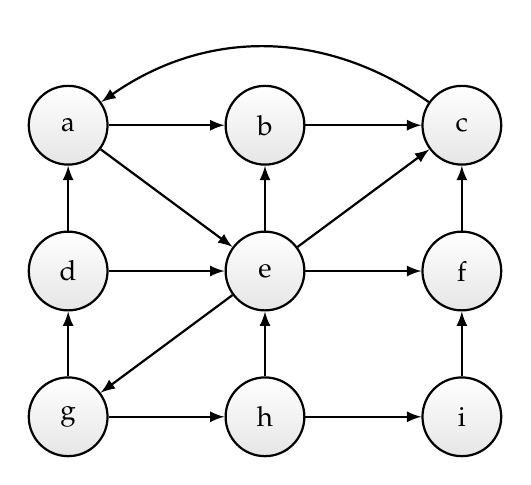
\begin{tikzpicture}[>= latex, node distance = 1.5 cm and 2.5cm,on grid, thick,state/.style ={circle,top color =white,bottom color = gray!20,draw,black,text=black,minimum width =1.0 cm}]
\node[state] (a) {a};
\node[state] (b) [right =of a] {b};
\node[state] (c) [right =of b] {c};
\node[state] (d) [below =of a, yshift=-10] {d};
\node[state] (e) [right =of d] {e};
\node[state] (f) [right =of e] {f};
\node[state] (g) [below =of d, yshift=-10] {g};
\node[state] (h) [right =of g] {h};
\node[state] (i) [right =of h] {i};
\tikzset{every node/.style={fill=white}} 
\path[->] 	(a) edge  				(b)
		(a) edge				(e)
		(b) edge				(c)
		(c) edge [bend right=35]	(a)
		(d) edge				(a)
		(d) edge				(e)
		(e) edge				(b)
		(e) edge				(c)
		(e) edge				(f)
		(e) edge				(g)
		(f) edge				(c)
		(g) edge				(d)
		(g) edge				(h)
		(h) edge				(e)
		(h) edge				(i)
		(i) edge				(f);
\end{tikzpicture}
\end{center}
\end{figure}

Consider running depth-first search on this graph starting from node $a$.  When there are multiple choices for the next node to visit, go in alphabetical order.

\begin{enumerate}[label=(\alph*)]
\item  \textbf{(5 points)} Label every edge as either tree, forward, backward, or cross.

\solution \\

Lecture 15...

(a,b): forward \\
(a,e): tree \\

(b,c): cross \\

(c,a): cross \\

(d,a):\\
(d,e):\\

(e,b): tree\\
(e,c):\\
(e,f):\\
(e,g): tree \\

(f,c): tree \\

(g,h): tree\\
(g,d): tree\\

(h,e): \\
(h,i): tree \\

(i,f): tree \\

\item  \textbf{(5 points)} Give the discovery and finish times of all vertices

\solution \\ 

\begin{tabular}{||ccc||}
	Vertex & Discovery & Finish\\
	\hline
	a & 1 & 18 \\
	b & 15 & 16 \\
	c & 9 & 10 \\
	d & 4 & 5 \\
	e & 2 & 17 \\
	f & 8 & 11 \\ 
	g & 3 & 14 \\
	h & 6 & 13 \\ 
	i & 7 & 12 \\ 
\end{tabular}


\item  \textbf{(5 points)} Is this graph a DAG?  If so, give a topological ordering.

\solution \\ 
No, the exist no node that has $in\_degree(v) = 0$. Therefore, a cycle is in this graph, which a DAG cannot have being acyclic.



\end{enumerate}


\newpage

\begin{prob} Shortest Paths Practice  \emph{(10 points)} \end{prob}

Use Dijkstra's algorithm the single-source shortest path problem on the following graph, using node $1$ as the source node $s$.  Write the distance from $s$ to each node and the parent of each node in the shortest path tree in the skeleton table provided. Show your work in order to receive partial credit.

\vspace{15pt}
\begin{figure}[h!]
\begin{center}
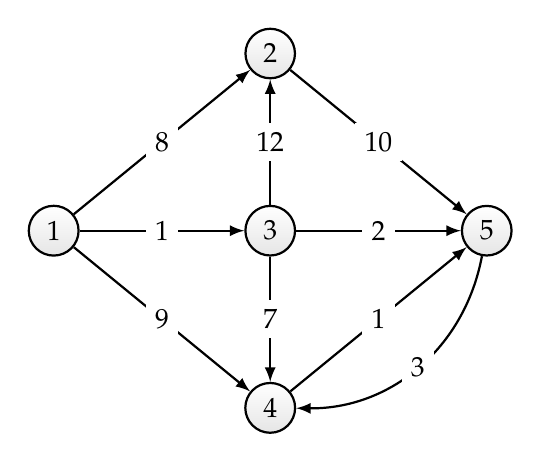
\begin{tikzpicture}[>= latex, node distance = 2.25 cm and 2.75cm,on grid, thick,state/.style ={circle,top color =white,bottom color = gray!20,draw,black,text=black,minimum width =.3 cm}]
\node[state] (a) {1};
\node[state] (b) [above right =of a] {2};
\node[state] (c) [right =of a] {3};
\node[state] (d) [below right =of a] {4};
\node[state] (e) [right =of c] {5};
\tikzset{every node/.style={fill=white}} 
\path[->] 	(a) edge node {8} (b)
		(a) edge node {9} (d)
		(a) edge node {1} (c);
\path[->] 	(b) edge node {10} (e);
\path[->]	(c) edge node {12} (b)
		(c) edge node {7} (d)
		(c) edge node {2} (e);
\path[->]	(d) edge node {1} (e);
\path[->]	(e) edge [bend left=40] node  {3} (d);
\end{tikzpicture}
\end{center}
\end{figure}

\vspace{15pt}
\solution
\vspace{15pt}

\begin{center}
\begin{tabular}{|l|c|c|c|c|c|}
\hline
Node & 1 & 2 & 3 & 4 & 5 \\
\hline
Distance & 0 & 8 & 1 & 6 & 3  \\
Parent   & $\emptyset$ & 1 & 1 & 4 & 3 \\
\hline
\end{tabular}
\end{center}

TODO ATTACH SCRATCH WORK

\end{document}
